\documentclass{article}\usepackage[]{graphicx}\usepackage[]{color}
%% maxwidth is the original width if it is less than linewidth
%% otherwise use linewidth (to make sure the graphics do not exceed the margin)

\makeatletter
\def\maxwidth{ %
  \ifdim\Gin@nat@width>\linewidth
    \linewidth
  \else
    \Gin@nat@width
  \fi
}
\makeatother

\usepackage{framed}
\makeatletter

\definecolor{fgcolor}{rgb}{0.345, 0.345, 0.345}
\newcommand{\hlnum}[1]{\textcolor[rgb]{0.686,0.059,0.569}{#1}}%
\newcommand{\hlstr}[1]{\textcolor[rgb]{0.192,0.494,0.8}{#1}}%
\newcommand{\hlcom}[1]{\textcolor[rgb]{0.678,0.584,0.686}{\textit{#1}}}%
\newcommand{\hlopt}[1]{\textcolor[rgb]{0,0,0}{#1}}%
\newcommand{\hlstd}[1]{\textcolor[rgb]{0.345,0.345,0.345}{#1}}%
\newcommand{\hlkwa}[1]{\textcolor[rgb]{0.161,0.373,0.58}{\textbf{#1}}}%
\newcommand{\hlkwb}[1]{\textcolor[rgb]{0.69,0.353,0.396}{#1}}%
\newcommand{\hlkwc}[1]{\textcolor[rgb]{0.333,0.667,0.333}{#1}}%
\newcommand{\hlkwd}[1]{\textcolor[rgb]{0.737,0.353,0.396}{\textbf{#1}}}%



\usepackage{framed}
\makeatletter
\newenvironment{kframe}{%
 \def\at@end@of@kframe{}%
 \ifinner\ifhmode%
  \def\at@end@of@kframe{\end{minipage}}%
  \begin{minipage}{\columnwidth}%
 \fi\fi%
 \def\FrameCommand##1{\hskip\@totalleftmargin \hskip-\fboxsep
 \colorbox{shadecolor}{##1}\hskip-\fboxsep
     % There is no \\@totalrightmargin, so:
     \hskip-\linewidth \hskip-\@totalleftmargin \hskip\columnwidth}%
 \MakeFramed {\advance\hsize-\width
   \@totalleftmargin\z@ \linewidth\hsize
   \@setminipage}}%
 {\par\unskip\endMakeFramed%
 \at@end@of@kframe}
\makeatother

\definecolor{shadecolor}{rgb}{.97, .97, .97}
\definecolor{messagecolor}{rgb}{0, 0, 0}
\definecolor{warningcolor}{rgb}{1, 0, 1}
\definecolor{errorcolor}{rgb}{1, 0, 0}
\newenvironment{knitrout}{}{} % an empty environment to be redefined in TeX

\usepackage{alltt}
\usepackage{fancyhdr}
\pagestyle{fancy}
\setlength{\parskip}{\smallskipamount}
\setlength{\parindent}{0pt}
\usepackage{amsthm}
\usepackage{amsmath}
\usepackage{wrapfig}
\usepackage{graphicx}
\usepackage{float}
\usepackage[margin=1in]{geometry}
\IfFileExists{upquote.sty}{\usepackage{upquote}}{}

\newtheorem{corollary}{Corollary}[section]
\newtheorem{theorem}{Theorem}
\newtheorem{example}{Example}
\newtheorem{question}{Question}
\newtheorem{remark}{Remark}[section]
\newtheorem{conjecture}{Conjecture}
\newtheorem{proposition}{Proposition}[section]
\newtheorem{definition}{Definition}[section]


\begin{document}


\title{Lab 4-Binary Classifier\\
Stat 215A, Fall 2014}

\author{PLEASE WRITE YXiang (Lisha) Li}

\maketitle


\section{Introduction}
Blah blah...

\section{EDA}
\subsection{Densities of the three most important features as selected by paper}



\begin{figure}[h]
\minipage{0.32\textwidth}
  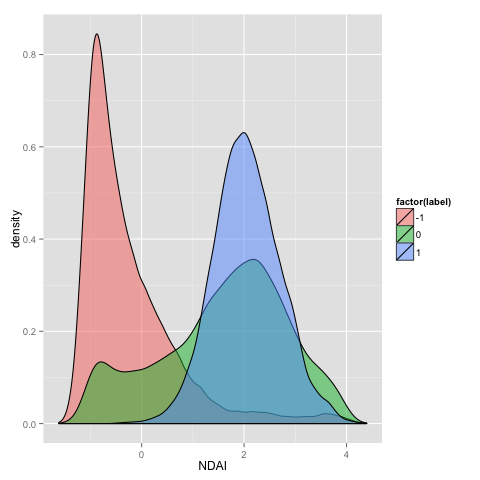
\includegraphics[width=\linewidth]{NDAI1.png}
  \caption{NDAI density Image 1}\label{}
\endminipage\hfill
\minipage{0.32\textwidth}
  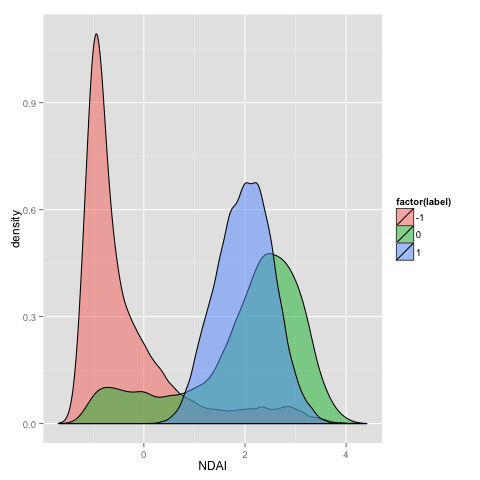
\includegraphics[width=\linewidth]{NDAI2.png}
  \caption{NDAI density Image 2}\label{}
\endminipage\hfill
\minipage{0.32\textwidth}%
  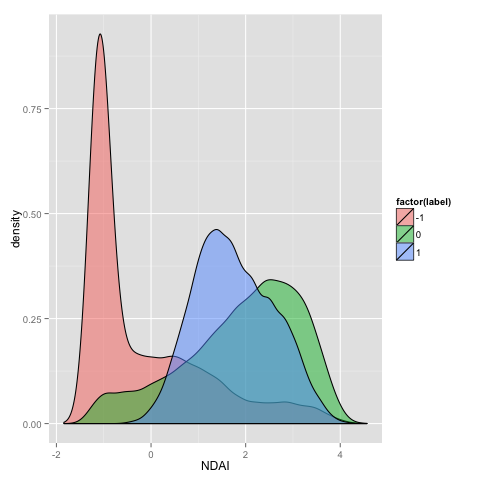
\includegraphics[width=\linewidth]{NDAI3.png}
  \caption{NDAI density Image 3}\label{}
\endminipage
\end{figure}

\begin{figure}[h]
\minipage{0.32\textwidth}
  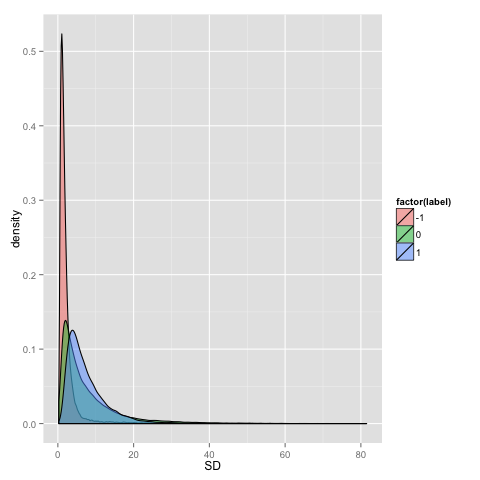
\includegraphics[width=\linewidth]{SD1.png}
  \caption{SD density Image 1}\label{}
\endminipage\hfill
\minipage{0.32\textwidth}
  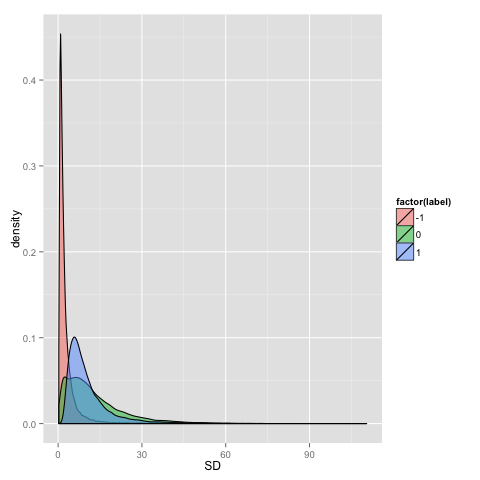
\includegraphics[width=\linewidth]{SD2.png}
  \caption{SD density Image 2}\label{}
\endminipage\hfill
\minipage{0.32\textwidth}%
  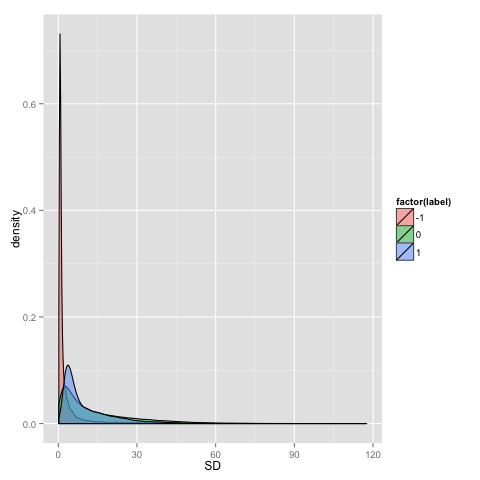
\includegraphics[width=\linewidth]{SD3.png}
  \caption{SD density Image 3}\label{}
\endminipage
\end{figure}


\begin{figure}[h]
\minipage{0.32\textwidth}
  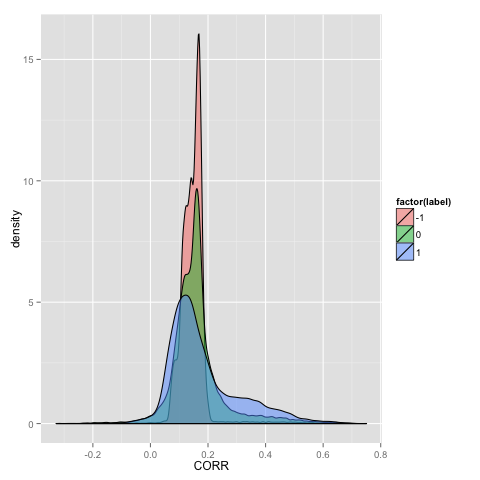
\includegraphics[width=\linewidth]{CORR1.png}
  \caption{CORR density Image 1}\label{}
\endminipage\hfill
\minipage{0.32\textwidth}
  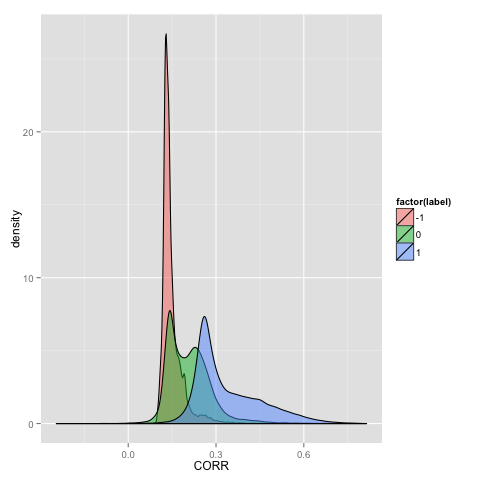
\includegraphics[width=\linewidth]{CORR2.png}
  \caption{CORR density Image 2}\label{}
\endminipage\hfill
\minipage{0.32\textwidth}%
  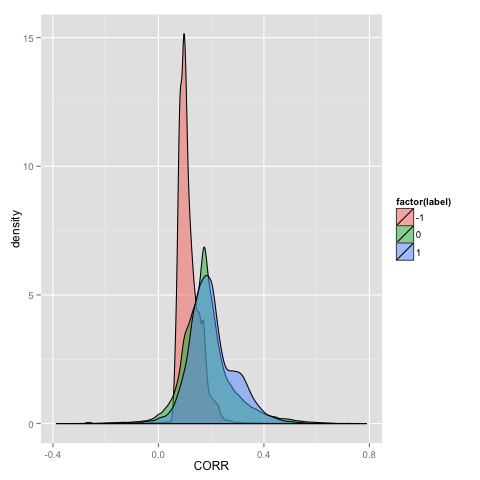
\includegraphics[width=\linewidth]{CORR3.png}
  \caption{CORR density Image 3}\label{}
\endminipage
\end{figure}




\section{Modeling}

\subsection{LDA/QDA}

\subsection{Logit/Probit}

\subsection{Random Forest}

\section{Reproducibility}

{\bf How we organized out code and github repo}


 \begin{thebibliography}{1}

\bibitem{notes} Ben-Hur, A., Elisseeff, A., Guyon, I.: A stability based method for discovering structure in clustered data. In: Pacific Symposium on Biocomputing, pp. 6�17.   
\end{thebibliography}


\end{document}